\section{Experimental evaluation}
\label{sec:results}
%todo: check entire section looking for overcomplex paragraphs or too many ideas in a single one
\subsection{Experimental setup and implementation details}

\subsubsection{Implementation and Hardware Details}
\label{sec:implementation_details}

The primary optimization infrastructure and the evolutionary many-objective engine are developed in Python, utilizing the \texttt{pymoo} optimization library~\cite{pymoo} to manage the uniform exploration and preference-guided genetic search paradigms, chromosome populations, reference direction meshes, and selection mechanics. 

Concurrently, all deep learning pipelines are powered by the \textit{PyTorch}~\cite{pytorch} ecosystem. Additionally, to improve runtime efficiency, the resulting layout coordinates for the solution~$\solution$ are  structured into a single unified sequence tensor, and evaluated by the PyTorch Transformer encoder in a single massive inference batch per generation. This mechanism restricts deep learning inference overhead to exactly one forward pass per evolutionary generation, significantly accelerating the algorithmic execution timeline.

The sequence-preserving prefix packing decoder (Algorithm~\ref{alg:packing_decoder}) and the exhaustive backtracking recursive spatial placement solver (Algorithm~\ref{alg:solve_recursive}) are fully implemented in native \textit{C++} since the decoding process is invoked many times per generation. To minimize algorithmic complexity and prevent concurrent race conditions during the search, the geometric packing routine processes individual candidate solutions sequentially. 

The computational environments are strictly partitioned according to their operational and memory demands:
\begin{itemize}
    \item Online Optimization: The evolutionary search, chromosome manipulations, and sequential backtracking packing evaluations were executed on a local workstation equipped with an 8-core CPU architecture and 32 GB of system RAM.
    
    \item Offline Training: The  training phase for the relational Transformer was conducted on the same dedicated high-performance GPU computing cluster node indicated in \secref{sec:gwes-implementation}.
\end{itemize}



\subsection{Historical dataset and instance setup}
\label{subsec:dataset_characterization}

To evaluate the architectural robustness and industrial applicability of the proposed framework, empirical validations were conducted using the \laprovence archive (\secref{sec:laprovence}). 

Real production archives are used, rather than synthetically generated instances, because this evaluation directly targets industrial applicability: synthetic instances could bias the benchmark toward artificial regularities absent from actual editorial practice, whereas real historical pages guarantee that both article content statistics and resulting layout complexity reflect genuine \melody\ production conditions. 
Moreover, since these pages were actually published, they are known a priori to admit a feasible single-page composition satisfying the constraints of \secref{sec:constraints_space}. Ensuring the same for synthetically generated instances would instead require substantially more filtering effort to guarantee that feasible, non-trivial solutions exist.

This dataset serves two purposes within this evaluation: it supplies the empirical objective distributions from which the historical aspiration vectors guiding the preference-based selection of \methodName are extracted, as detailed in \secref{sec:many-objective_optimization}; and it is utilized, together with the independent test set defined in \secref{sec:gwes}, to construct the evaluation problem instances~$\instance$ used to benchmark \methodName. Concurrently, the static template catalog~$\templatecatalog$ coming from the same newspaper group serves as part of the search domain for the evolutionary optimization engine.

\subsubsection*{Historical dataset for aspiration vectors}

The historical aspiration vectors used by \methodName\ (\secref{sec:many-objective_optimization}) are computed over the full set of $4{,}449$ usable \laprovence pages described in \secref{sec:dataset-preprocessing}.

\subsubsection*{Instance Setup}


An instance set comprising 30 instances was established. To ensure strict validation integrity and prevent data leakage with \neuralmethod, these instances were sampled from the intersection of the exact-match and admissible-elasticity categories described in \secref{sec:dataset-preprocessing} ($2{,}775$ pages) and the independent test set defined in \secref{sec:gwes}. The experimental corpus covers a wide spectrum of visual complexities by varying the number of articles per page, ranging from low-density configurations to a practical upper bound in \melody. The structural distribution of the instance setup is detailed in Table~\ref{tab:instance_distribution}.

\begin{table}[htbp]
\centering
\begin{tabularx}{\linewidth}{Xcc}
\hline
\textbf{Complexity} & \textbf{Articles per Page ($\numarticles$)} & \textbf{Instance Count} \\ \hline
Low Density & 2 & 7 \\
            & 3 & 7 \\ \hline
Medium Density & 4 & 10 \\
               & 5 & 4 \\ \hline
High Density   & 6 & 1 \\
               & 8 & 1 \\ \hline
\textbf{Total Number of Instances} & & \textbf{30} \\ \hline
\end{tabularx}
\caption{Structural composition and article density distribution of the 30 production layout instances utilized.}
\label{tab:instance_distribution}
\end{table}

As shown in Table~\ref{tab:instance_distribution}, these instances are grouped into strata by their number of articles $\numarticles$, since their difficulty and objective magnitudes scale directly with this quantity. All results reported in the following sections are therefore stratified by $\numarticles$.
The sample frequencies for $n=6$ and $n=8$ reflect the exact availability limits within the  test set, rather than an arbitrary choice. The evaluation ceiling is strictly capped at $n=8$ articles, since layouts exceeding this threshold represent editorial edge cases that fall outside the operational scope of the required task.

To account for the stochastic nature of the evolutionary operators and ensure statistical significance, all comparative experiments across the 30 benchmark instances were executed over 30 independent runs, each utilizing a unique random seed.


\begin{callout}
Note that for each selected instance, the geometric coordinates, positions, and final template allocations selected by human designers were completely stripped from the metadata. The baseline models and the evolutionary framework were provided exclusively with the article's content and constraints that define the formal input vector $\instance = \langle \page, \articleset \rangle$.  This configuration forces a true blind evaluation, challenging the algorithms to generate layouts purely from raw content specifications.
\end{callout}



%%%%%%%%% Hyperparameters U%%%%%%%%%%%%%
\subsection{Hyperparameter configuration}
\label{subsec:hyperparameter_calibration}

The operational parameters governing the evolutionary engine were set following two distinct procedures, depending on their nature, as structured in Table~\ref{tab:algorithmic_parameters}. The domain-specific coefficients were validated through focus-groups conducted with \melody experts, ensuring their alignment with established editorial practice, with the exception of the LayoutGMN kernel smoothing parameter $\sigmagmn$, which was instead set empirically according to the dataset characteristics (\secref{sec:gwes-gmn-mapping}); the remaining evolutionary hyperparameters governing the NSGA-III/RNSGA-III search were manually set through extensive empirical pilot studies and operational stress tests.

\begin{table}[htbp]
\centering

\begin{tabularx}{\textwidth}{@{}l l X l@{}}
\toprule
Category & Symbol & Parameter Description & Value \\
\midrule
\multirow{9}{*}{\makecell[l]{Domain-specific \\ Coefficients}}
           & $\elasticityset$ & Elasticity set & $\{-15, -10, -5, 0, 5, 10, 15\}$ \\
           & $\objthreeepsilon$ & Epsilon tolerance for \objthree & 0.1 \\
           & $\betaweight$ & Weight parameter for \objfour & 0.5 \\
           & $\Klower$ & Lower capacity text penalty coef. & 5 \\
           & $\Kupper$ & Upper capacity text penalty coef. & 10 \\
           & $\alignmentScalingParameter$ & Edge-alignment scaling parameter & 5 \\
           & $\threshalignlower$ & Lower threshold for alignment penalization zone & 0.006 \\
           & $\threshalignupper$ & Upper threshold for alignment penalization zone & 0.3 \\
           & $\sigmagmn$ & LayoutGMN kernel smoothing parameter & 0.5 \\
\midrule
\multirow{13}{*}{\makecell[l]{NSGA-III /  RNSGA-III \\hyperparameters}}
           & --- & Number of reference directions for \methodNameUniform & 10 \\
           & $\popsize$ & Population size for \methodNameUniform & 286 \\
           & $\RNSGAradius$ & Local mesh contraction factor in \methodName & 0.15 \\
           & $\popsize_{R}$ & Total population size for \methodName & 330 \\
           & $\ngen$ & Number of generations & 300 \\
           & $p_{\text{cross}}$ & Crossover probability & 0.5 \\
           & $\globalmutationprob$ & Global mutation probability & 0.4 \\
           & $\mutationprob{1}$ & Perm. reverse mutation prob. & 0.2 \\
           & $\mutationprob{2}$ & 5-most similar template mutation prob. & 0.25 \\
           & $\mutationprob{3}$ & Textual integrity mutation prob. & 0.25 \\
           & $\mutationprob{4}$ & Bernoulli resampling mutation prob. & 0.05 \\
           & $\mutationprob{5}$ & Random template substitution mutation prob. & 0.05 \\
           & $\mutationprob{6}$ & Elasticity mutation prob. & 0.2 \\
\bottomrule
\end{tabularx}

\caption{Domain-specific coefficients and evolutionary hyperparameters for the \methodName\ method.}
\label{tab:algorithmic_parameters}
\end{table}

The asymmetric population sizes reported in Table~\ref{tab:algorithmic_parameters} ($\popsize = 286$ versus $\popsize_R = 330$) are not arbitrary hyperparameter selections; rather, they are strictly dictated by the underlying combinatorial requirements of the reference direction generation methods inside the \texttt{pymoo} framework:
\begin{enumerate}
    \item For \methodNameUniform, deploying the canonical Das-Dennis boundary intersection method with $10$ structured partitions across the $4$-dimensional objective space mathematically yields exactly $\binom{4 + 10 - 1}{10} = 286$ unique reference vectors, necessitating an identical population size to guarantee niche coverage. 
    \item Conversely, \methodName\ projects a structured mesh of $8$ internal partitions around each of the $2$ extracted historical aspiration points (the 25th and 50th percentiles of empirical human designs), which generates exactly $165$ localized reference lines per target zone, culminating in a combined population tracking space of $165 \times 2 = 330$ individuals to preserve directional diversity. The deliberate selection of $8$ internal partitions for the preference-guided approach was specifically enforced to maintain an equitable computational budget and search capacity per generation, thereby ensuring a balanced comparative analysis between both paradigms.
\end{enumerate}


%%%%%%%%%%%%%%%%%%%% Results %%%%%%%%%%%%%%%%%%%%%%%%%%%%%%%%%%%%%%%%%%%%%%%



%%%%%%%%%%%%%%%%%%%% NSGA ANALYSIS %%%%%%%%%%%%%%%%%%%%%

\subsection{Comparison with alternative baselines}

This subsection presents a quantitative evaluation of \methodNameUniform, the uniform variant of \methodNameGeneral, against the decoupled baselines described below. The uniform variant is evaluated first because it makes no assumptions about historical editorial preferences, making it the fairest basis for comparison against these baselines; the preference-guided variant \methodName\ is compared directly against \methodNameUniform\ separately in \secref{sec:rnsga-vs-nsga}.

\subsubsection{Baseline Methods}
\label{subsubsec:baselines}

To validate the performance of the integrated \methodNameUniform\ method, five competitive baselines ($\baseline{1}$ to $\baseline{5}$) were constructed. These models isolate different architectural paradigms. Three of them ($\baseline{2}$--$\baseline{4}$) follow a \emph{decoupled} sequential paradigm: template selection and spatial packing are solved as two independent sub-problems, each resolved with a technique that is best suited to it in isolation, rather than jointly optimized as in \methodNameGeneral. As shown below, however, this apparent advantage does not hold once both sub-problems interact. The baselines are formally defined below:
\begin{description}
    \item[$\baseline{1}$ (Blind Random with Bottom-Left Packer):] Establishes the absolute lower bound of performance. It processes articles using their canonical entry order and assigns random feasible templates from the catalog $\templatecatalog$. Elasticity is fixed to 0. Packing is executed via a traditional Top-Left heuristic, which is simply Bottom-Left~\cite{chazelle-bl} but mirrored vertically.
    
    \item[$\baseline{2}$ (Heuristic Selection with Fixed Order):] A decoupled sequential approach. Template selection is purely deterministic, choosing the feasible candidate that minimizes the text capacity penalty ($\objthree$) in isolation. Articles are packed using their canonical entry order  using the packing decoder engine, the same that \methodNameUniform\ uses.
    
    \item[$\baseline{3}$ (Heuristic Selection with Exact Permutation Backtracking):] Another decoupled sequential approach. Template selection isolates and minimizes $\objthree$. For the packing stage, an exact backtracking search evaluates all $\numarticles!$ article permutations, minimizing a scalarized fitness function defined as $W = 4\objone + \objtwo + 0\objthree + 4\objfour$. Setting the weight of $\objthree$ to 0 avoids redundant optimization, while $\objtwo$ is minimized as a low-priority target given the fixed templates. This assigns equal dominant weight to $\objone$ and $\objfour$, mirroring the implicit balancing mechanism of \methodNameUniform. Elasticity is fixed to 0, and packing is handled by the packing decoder engine.
    
    \item[$\baseline{4}$ (Transformer-Assisted Selection with Exact Backtracking):] A decoupled sequential approach enhanced by deep learning. Template selection is guided by the Top-1 probabilities of the Transformer Encoder, previously filtered by a Top-$K$ text-capacity threshold ($\objthree$). The parameter $K$ is set to $0.2$ (retaining the top 20\% best candidates), balancing neural design exploration with structural heuristic text integrity safety. Packing executes the exact permutation backtracking as in $\baseline{3}$, with zero elasticity over the packing decoder engine.
    
    \item[$\baseline{5}$ (Ablated NSGA-III):] A simultaneous (non-decoupled) optimization baseline that shares the exact mechanisms as the proposed \methodNameUniform, but acts as a structural ablation by deactivating the template editorial style objective $\objtwo$.
\end{description}

Table~\ref{tab:pagegen_baselines_summary} summarizes the key features that distinguish these baselines from the proposed \methodNameUniform.

\begin{table}[htbp]
    \centering
    \begin{tabular}{lccccc}
        \toprule
        \textbf{Method} & \textbf{HS} & \textbf{JT} & \textbf{EO} & \textbf{NS} & \textbf{MO} \\
        \midrule
        $\baseline{1}$          & $\times$     & $\times$     & $\times$     & $\times$     & $\times$    \\
        $\baseline{2}$          & $\checkmark$ & $\times$     & $\times$     & $\times$     & $\times$    \\
        $\baseline{3}$          & $\checkmark$ & $\times$     & $\checkmark$ & $\times$     & $\times$    \\
        $\baseline{4}$          & $\times$     & $\times$     & $\checkmark$ & $\checkmark$ & $\times$    \\
        $\baseline{5}$          & --           & $\checkmark$ & --           & $\times$     & $\checkmark$ \\
        \methodNameUniform      & --           & $\checkmark$ & --           & $\checkmark$ & $\checkmark$ \\
        \bottomrule
    \end{tabular}
    \caption{
    Comparison of features across baseline methods and \methodNameUniform.
    Abbreviations: HS = heuristic template selection (deterministic, minimizes text capacity penalty $\objthree$); JT = joint template-and-packing optimization, rather than a decoupled sequential paradigm; EO = exhaustive/exact search over article ordering; NS = uses \neuralmethod to guide template selection; MO = outputs a full multi-objective Pareto frontier rather than a single solution. A dash (--) indicates that the criterion does not apply.}
    \label{tab:pagegen_baselines_summary}
\end{table}

\subsubsection{Compromise-Solution Evaluation: Multi-Objective Methods vs. Decoupled Single-Solution Baselines}

Unlike  decoupled approaches that yield a single solution, multi-objective evolutionary algorithms preserve a diverse set of trade-offs along a Pareto frontier. To perform a fair quantitative comparison against single-solution baselines ($\baseline{1}$ to $\baseline{4}$), a representative decision-making vector must be extracted from the non-dominated sets generated by the Ablated NSGA-III ($\baseline{5}$) and the proposed \methodNameUniform. For this purpose, the compromise-solution formulation was selected.


Mathematically, the compromise solution represents the best trade-off within a Pareto frontier. Geometrically, because all objective functions ($\objone, \objtwo, \objthree, \objfour$) are formulated as minimization targets, it is strictly defined as the solution with the minimum normalized euclidean distance to the ideal point, normalized component-wise using the ideal and nadir points introduced in \secref{sec:sota-pareto} as bounds for each objective. Since every objective in $\objvector$ is a non-negative penalty whose theoretical optimum is zero, the ideal point reduces here to $z^\ast = (0, 0, 0, 0)$. The macro-aggregated objective scores across the different \numarticles strata are summarized in Table~\ref{tab:compromise_solution_metrics}.


\begin{table}[htbp]
\centering
\begin{tabular}{lllllll}
\toprule
$\numarticles$ & Method & $N_{pages}$ & \objone & \objthree & \objfour & \objtwo \\
\midrule
\multirow[c]{6}{*}{2} & B1 & \cellcolor{red!15}1.62 $\pm$ 0.49 & 0.81 $\pm$ 0.31 & 1.89 $\pm$ 1.67 & 0.38 $\pm$ 0.25 & 1.71 $\pm$ 0.37 \\
 & B2 & \bfseries1.00 $\pm$ 0.00 & 0.29 $\pm$ 0.10 & \cellcolor{green!15}\bfseries0.00 $\pm$ 0.00 & 0.59 $\pm$ 0.13 & 1.87 $\pm$ 0.17 \\
 & B3 & \bfseries1.00 $\pm$ 0.00 & \cellcolor{green!15}0.29 $\pm$ 0.10 & \cellcolor{green!15}\bfseries0.00 $\pm$ 0.00 & 0.59 $\pm$ 0.13 & 1.84 $\pm$ 0.17 \\
 & B4 & \cellcolor{red!15}1.14 $\pm$ 0.35 & 0.30 $\pm$ 0.30 & 0.11 $\pm$ 0.07 & \cellcolor{green!15}0.05 $\pm$ 0.12 & \cellcolor{green!15}1.41 $\pm$ 0.44 \\
 & B5 & \bfseries1.00 $\pm$ 0.00 & \cellcolor{green!15}\bfseries 0.02 $\pm$ 0.04 & \cellcolor{green!15}0.11 $\pm$ 0.16 & \cellcolor{green!15}\bfseries0.00 $\pm$ 0.00 & \cellcolor{green!15}1.10 $\pm$ 0.36 \\
 & \methodNameUniform & \bfseries1.00 $\pm$ 0.00 & \cellcolor{green!15}0.04 $\pm$ 0.07 & 0.18 $\pm$ 0.13 & \cellcolor{green!15}0.01 $\pm$ 0.05 & \cellcolor{green!15}\bfseries0.32 $\pm$ 0.17 \\
  \hline
\multirow[c]{6}{*}{3} & B1 & \cellcolor{red!15}2.28 $\pm$ 0.73 & 1.11 $\pm$ 0.48 & 2.37 $\pm$ 1.38 & 0.47 $\pm$ 0.30 & 2.55 $\pm$ 0.41 \\
 & B2 & \cellcolor{red!15}1.14 $\pm$ 0.35 & 0.36 $\pm$ 0.36 & \cellcolor{green!15}\bfseries0.00 $\pm$ 0.00 & 0.66 $\pm$ 0.18 & 2.56 $\pm$ 0.28 \\
 & B3 & \cellcolor{red!15}1.14 $\pm$ 0.35 & \cellcolor{green!15}0.36 $\pm$ 0.36 & \cellcolor{green!15}\bfseries0.00 $\pm$ 0.00 & 0.66 $\pm$ 0.18 & 2.50 $\pm$ 0.28 \\
 & B4 & \cellcolor{red!15}1.57 $\pm$ 0.50 & 0.81 $\pm$ 0.45 & \cellcolor{green!15}0.19 $\pm$ 0.18 & \cellcolor{green!15}0.38 $\pm$ 0.31 & \cellcolor{green!15}1.92 $\pm$ 0.38 \\
 & B5 & \bfseries1.00 $\pm$ 0.00 & \cellcolor{green!15}0.04 $\pm$ 0.03 & 0.29 $\pm$ 0.40 & \cellcolor{green!15}0.14 $\pm$ 0.20 & \cellcolor{green!15}1.60 $\pm$ 0.40 \\
 & \methodNameUniform & \bfseries1.00 $\pm$ 0.00 & \cellcolor{green!15}\bfseries0.04 $\pm$ 0.02 & 0.26 $\pm$ 0.13 & \cellcolor{green!15}\bfseries0.09 $\pm$ 0.13 & \cellcolor{green!15}\bfseries0.64 $\pm$ 0.23 \\
   \hline
\multirow[c]{6}{*}{4} & B1 & \cellcolor{red!15}2.87 $\pm$ 0.82 & 1.39 $\pm$ 0.49 & 2.58 $\pm$ 0.96 & 0.54 $\pm$ 0.33 & 3.43 $\pm$ 0.47 \\
 & B2 & \cellcolor{red!15}1.40 $\pm$ 0.49 & 0.65 $\pm$ 0.45 & 3.12 $\pm$ 0.38 & 0.65 $\pm$ 0.16 &\cellcolor{green!15}\bfseries 0.01 $\pm$ 0.03 \\
 & B3 & \cellcolor{red!15}1.40 $\pm$ 0.49 & \cellcolor{green!15}0.65 $\pm$ 0.45 & \cellcolor{green!15}\bfseries0.01 $\pm$ 0.03 & 0.65 $\pm$ 0.16 & 2.85 $\pm$ 0.35 \\
 & B4 & \cellcolor{red!15}1.50 $\pm$ 0.50 & 0.68 $\pm$ 0.50 & 0.85 $\pm$ 0.33 & \cellcolor{green!15}0.53 $\pm$ 0.26 & \cellcolor{green!15}2.34 $\pm$ 0.42 \\
 & B5 & \bfseries1.00 $\pm$ 0.00 & \cellcolor{green!15}\bfseries0.06 $\pm$ 0.03 & \cellcolor{green!15}0.38 $\pm$ 0.42 & \cellcolor{green!15}0.23 $\pm$ 0.23 & 2.55 $\pm$ 0.51 \\
 & \methodNameUniform & \bfseries1.00 $\pm$ 0.00 & \cellcolor{green!15}0.08 $\pm$ 0.03 & \cellcolor{green!15}0.44 $\pm$ 0.27 & \cellcolor{green!15}\bfseries0.23 $\pm$ 0.15 & \cellcolor{green!15}\bfseries1.24 $\pm$ 0.32 \\
  \hline
\multirow[c]{6}{*}{5} & B1 & \cellcolor{red!15}3.54 $\pm$ 0.98 & 1.70 $\pm$ 0.62 & 2.81 $\pm$ 0.81 & 0.56 $\pm$ 0.32 & 4.33 $\pm$ 0.47 \\
 & B2 & \cellcolor{red!15}1.50 $\pm$ 0.50 & 0.68 $\pm$ 0.48 & \cellcolor{green!15}\bfseries0.07 $\pm$ 0.09 & 0.83 $\pm$ 0.04 & 4.00 $\pm$ 0.33 \\
 & B3 & \cellcolor{red!15}1.50 $\pm$ 0.50 & 0.68 $\pm$ 0.48 & \cellcolor{green!15}\bfseries0.07 $\pm$ 0.09 & 0.81 $\pm$ 0.06 & \cellcolor{green!15}3.39 $\pm$ 0.32 \\
 & B4 & \cellcolor{red!15}1.50 $\pm$ 0.50 & \cellcolor{green!15}0.63 $\pm$ 0.37 & 1.37 $\pm$ 0.32 & \cellcolor{green!15}0.50 $\pm$ 0.12 & \cellcolor{green!15}2.26 $\pm$ 0.37 \\
 & B5 & \bfseries1.00 $\pm$ 0.00 & \cellcolor{green!15}\bfseries0.06 $\pm$ 0.04 & 0.77 $\pm$ 0.63 & \cellcolor{green!15}0.35 $\pm$ 0.27 & 3.46 $\pm$ 0.54 \\
 & \methodNameUniform & \bfseries1.00 $\pm$ 0.00 & \cellcolor{green!15}0.08 $\pm$ 0.03 & \cellcolor{green!15}0.49 $\pm$ 0.27 & \cellcolor{green!15}\bfseries0.26 $\pm$ 0.16 & \cellcolor{green!15}\bfseries1.85 $\pm$ 0.46 \\
  \hline
\multirow[c]{6}{*}{6} & B1 & \cellcolor{red!15}4.10 $\pm$ 1.09 & 1.94 $\pm$ 0.64 & 3.01 $\pm$ 0.63 & 0.57 $\pm$ 0.33 & 5.22 $\pm$ 0.46 \\
 & B2 & \cellcolor{red!15}2.00 $\pm$ 0.00 & 1.22 $\pm$ 0.00 & \cellcolor{green!15}\bfseries0.00 $\pm$ 0.00 & 0.51 $\pm$ 0.00 & 4.86 $\pm$ 0.00 \\
 & B3 & \cellcolor{red!15}2.00 $\pm$ 0.00 & 1.22 $\pm$ 0.00 & \cellcolor{green!15}\bfseries0.00 $\pm$ 0.00 & 0.51 $\pm$ 0.00 & \cellcolor{green!15}4.67 $\pm$ 0.00 \\
 & B4 & \cellcolor{red!15}2.00 $\pm$ 0.00 & \cellcolor{green!15}1.06 $\pm$ 0.00 & 1.41 $\pm$ 0.00 & \cellcolor{green!15}0.34 $\pm$ 0.00 & \cellcolor{green!15}4.03 $\pm$ 0.00 \\
 & B5 & \bfseries1.00 $\pm$ 0.00 & \cellcolor{green!15}\bfseries0.06 $\pm$ 0.04 & 0.73 $\pm$ 0.56 & \cellcolor{green!15}\bfseries0.24 $\pm$ 0.22 & 4.91 $\pm$ 0.51 \\
 & \methodNameUniform & \bfseries1.00 $\pm$ 0.00 & \cellcolor{green!15}0.12 $\pm$ 0.02 & \cellcolor{green!15}0.44 $\pm$ 0.24 & \cellcolor{green!15}0.26 $\pm$ 0.16 &\cellcolor{green!15}\bfseries 2.44 $\pm$ 0.51 \\
  \hline
\multirow[c]{6}{*}{8} & B1 & \cellcolor{red!15}4.63 $\pm$ 1.38 & 2.07 $\pm$ 0.79 & 3.25 $\pm$ 0.73 & 0.57 $\pm$ 0.30 & 7.02 $\pm$ 0.63 \\
 & B2 & \cellcolor{red!15}2.00 $\pm$ 0.00 & 1.15 $\pm$ 0.00 & \cellcolor{green!15}\bfseries0.00 $\pm$ 0.00 & 0.60 $\pm$ 0.00 & 5.94 $\pm$ 0.00 \\
 & B3 & \cellcolor{red!15}2.00 $\pm$ 0.00 & 1.15 $\pm$ 0.00 & \cellcolor{green!15}\bfseries0.00 $\pm$ 0.00 & 0.60 $\pm$ 0.00 & 5.87 $\pm$ 0.00 \\
 & B4 & \bfseries1.00 $\pm$ 0.00 & \cellcolor{green!15}0.10 $\pm$ 0.00 & 1.41 $\pm$ 0.00 & \cellcolor{green!15}\bfseries0.17 $\pm$ 0.00 & \cellcolor{green!15}\bfseries1.25 $\pm$ 0.00 \\
 & B5 & \bfseries1.00 $\pm$ 0.00 & \cellcolor{green!15}0.09 $\pm$ 0.05 & 0.54 $\pm$ 0.78 & \cellcolor{green!15}0.30 $\pm$ 0.24 & \cellcolor{green!15}5.53 $\pm$ 0.77 \\
 & \methodNameUniform & \bfseries1.00 $\pm$ 0.00 & \cellcolor{green!15}\bfseries0.08 $\pm$ 0.01 & \cellcolor{green!15}0.20 $\pm$ 0.10 & \cellcolor{green!15}0.18 $\pm$ 0.04 & \cellcolor{green!15}2.25 $\pm$ 0.46 \\
\bottomrule
\end{tabular}

\caption{Quantitative compromise-solution evaluation of multi-objective methods ($\baseline{5}$ and \methodNameUniform) against decoupled single-solution baselines ($\baseline{1}$--$\baseline{4}$) across different article counts ($\numarticles$). Metrics express the $\text{mean} \pm \text{standard deviation}$ computed over all runs and instances in the corresponding stratum. Bold entries indicate the best-performing method within each complexity tier for each individual objective (all formulated as minimization targets). Green-shaded cells mark the three best-performing methods per objective and stratum. Red-shaded $N_{pages}$ cells flag configurations that exceed a single page.}
\label{tab:compromise_solution_metrics}
\end{table}

The aggregated scores in Table~\ref{tab:compromise_solution_metrics} highlight the structural limitations of sequential design. While the evolutionary approaches ($\baseline{5}$ and \methodNameUniform) maintain absolute number of pages feasibility ($1.00 \pm 0.00$), the decoupled backtracking baselines ($\baseline{3}$ and $\baseline{4}$) frequently overflow into two pages as article density scales ($n \ge 6$). Even though $\baseline{3}$ and $\baseline{4}$ utilize exact permutation searches to minimize \objone, freezing the template selection beforehand forces the packing engine to operate over a fundamentally flawed geometric space, proving that decoupled pipelines cannot guarantee basic number of pages feasibility. A Friedman test confirms this variation is significant ($\chi^2 = 104.39, p < 0.001$, effect size $W = 0.70$) . Post-hoc Wilcoxon signed-rank tests with Bonferroni correction indicate no statistically significant difference between $\baseline{5}$ and \methodNameUniform\ in page counts.

When evaluating the entire objective space $\objvector$, a clear and strong trade-off effect characterizes the decoupled baselines ($\baseline{2}$, $\baseline{3}$, and $\baseline{4}$). These methods excel in isolated dimensions but collapse in others: $\baseline{2}$ and $\baseline{3}$ achieve near-perfect text capacity ($\objthree \approx 0.00$) at the expense of editorial styling ($\objtwo$), whereas $\baseline{4}$ improves $\objtwo$ but sacrifices text integrity ($\objthree$). Conversely, the simultaneous optimization paradigm proves its structural superiority through both the ablated baseline ($\baseline{5}$) and the proposed \methodNameUniform\ method, as both maintain a stable, harmonic balance across their active targets. While $\baseline{5}$ naturally exhibits high penalty scores in $\objtwo$ by design, since it serves as an ablation with this specific objective deactivated, it closely mirrors the proposed method in achieving exceptional scores in all objectives, validating the core strength of population-based multi-objective search.

This global behavior is validated by the Friedman test across $\objone$ ($\chi^2 = 126.16, p < 0.001, W = 0.84$), $\objtwo$ ($\chi^2 = 117.68, p < 0.001, W = 0.78$), $\objthree$ ($\chi^2 = 126.44, p < 0.001, W = 0.84$), and $\objfour$ ($\chi^2 = 119.25, p < 0.001, W = 0.80$). Pairwise post-hoc comparisons confirm that \methodNameUniform\ significantly outperforms $\baseline{5}$ in editorial historical alignment ($\objtwo$), while $\baseline{5}$ holds a slight but significant advantage in minimizing $\objone$. No statistically significant differences are detected between them for $\objthree$ and $\objfour$.


\subsubsection{Pareto Dominance over Decoupled Single-Solution Baselines}


To formally assess the multi-objective superiority of \methodNameUniform, the generated fronts are evaluated using the criterion of Pareto dominance, already introduced in \secref{sec:sota-pareto}. Applied to this multi-objective minimization problem governed by the objective vector $\objvector$, a solution  $\solution_A$ strictly dominates another one $\solution_B$ ($\solution_A \succ \solution_B$) if and only if:

\begin{equation}
\forall i \in \{1, \dots, 4\}: f_i(\solution_A) \le f_i(\solution_B) \quad \land \quad \exists j \in \{1, \dots, 4\}: f_j(\solution_A) < f_j(\solution_B).
\end{equation}

By mapping the single-solution outputs produced by the decoupled baselines ($\baseline{1}$ to $\baseline{4}$) against the non-dominated frontiers of \methodNameUniform, this verification determines whether the evolutionary search yields layout alternatives that are unconditionally superior, improving at least one objective without degrading any other.

Table~\ref{tab:pareto_dominance_metrics} reports, for each baseline and article count, the percentage of optimization runs in which \methodNameUniform's frontier contains at least one solution that Pareto-dominates the corresponding baseline output.
\begin{table}[htbp]
\centering
\begin{tabular}{lllll}
\toprule
$\numarticles$& $\baseline{1}$ & $\baseline{2}$ & $\baseline{3}$ & $\baseline{4}$ \\
\midrule
2 & 99.5\% & 95.2\% & 95.2\% & 94.8\% \\
3 & 99.5\% & 99.0\% & 99.0\% & 99.5\% \\
4 & 93.3\% & 95.7\% & 91.3\% & 99.7\% \\
5 & 91.7\% & 97.5\% & 84.2\% & 99.2\% \\
6 & 96.7\% & 73.3\% & 70.0\% & 100.0\% \\
8 & 96.7\% & 100.0\% & 100.0\% & 13.3\% \\
\bottomrule
\end{tabular}

\caption{Pareto dominance of \methodNameUniform\ over decoupled single-solution baselines. Percentage of optimization runs (seeds) where the multi-objective methods successfully discover solutions that dominate the decoupled baselines ($\baseline{1}$--$\baseline{4}$), stratified by article count ($n$).}
\label{tab:pareto_dominance_metrics}
\end{table}

An examination of the empirical results in Table~\ref{tab:pareto_dominance_metrics} reveals that the proposed \methodNameUniform\ method establishes near-absolute dominance over decoupled methods. For all configurations up to $\numarticles = 6$, the stability rates consistently hover between 70.0\% and 100.0\%,  confirming that the multi-objective search engine reliably discovers layouts that strictly outperform the isolated heuristics across all objectives at once.

The only notable exception occurs at the highest complexity stratum ($\numarticles = 8$), where the dominance rate against $\baseline{4}$ drops to 13.3\%. As shown in the compromise-solution analysis (Table~\ref{tab:compromise_solution_metrics}), $\baseline{4}$'s Transformer-driven template selection concentrates on \objtwo, outperforming \methodNameUniform\ along that single objective and thereby escaping Pareto dominance. However, \methodNameUniform\ still significantly outperforms $\baseline{4}$ in text capacity ($\objthree$) and wasted space ($\objone$), so $\baseline{4}$ does not offer a genuinely balanced alternative.

\subsubsection{Comparison between $\baseline{5}$ and \methodNameUniform}

To isolate and quantify the exact architectural contribution of the deep learning component within the optimization engine, a rigorous ablation analysis is conducted between the ablated method ($\baseline{5}$) and the proposed \methodNameUniform. Since both methods operate under the multi-objective paradigm and generate full Pareto frontiers rather than single solutions, traditional scalar metrics are insufficient. Instead, their performance is evaluated directly in their multi-objective domain using the Hypervolume (HV) indicator~\cite{hv}.

Intuitively, HV measures how much of the objective space a frontier covers toward improvement. Formally, a reference point $z^{\text{ref}}$ is fixed once, slightly worse than every objective's worst attainable value. Then, every solution in a frontier $A$ dominates the box of objective space delimited by itself and $z^{\text{ref}}$, and $HV(A)$ is the volume of the union of all these boxes across the frontier, $HV(A) = \Lambda\big(\bigcup_{a \in A} [a, z^{\text{ref}}]\big)$, where $\Lambda$ denotes that volume (the Lebesgue measure). A frontier that is both closer to the true Pareto frontier and more spread out across it covers a larger volume under this construction, so HV captures convergence and diversity jointly in a single number, where higher is always better. In this evaluation, $z^{\text{ref}}$ is set component-wise to $1.1$ times the empirical nadir point observed across the compared frontiers, i.e., $10\%$ beyond the worst value attained by each objective, a common convention in the field for fixing a reference point that remains slightly outside every attainable frontier, ensuring HV never collapses to zero and stays comparable across runs~\cite{ishibuchi-2018}.

%todo: figure to show hypervolume, based exactly on the figure in chapter 2 SOTA

\paragraph{Convergence}

First, it is necessary to evaluate the overall convergence of both evolutionary approaches. \figref{fig:convergence_analysis} tracks the hypervolume evolution over $\ngen = 300$ generations for a representative large-scale instance ($\numarticles = 8$).




\begin{figure}[htbp]
\centering
%todo: show also convergence curve of 4 articles or 5
%todo IMPORTANT THIS REQUIRE RE CHECKING THE CODE OF ANALYSIS.  CHECK THIS GRAPH IN CODE FOR SOME REASON IT DOES NOT FOLLOW THE TABLE
%todo: show better three cases (b5, methodname, and methodname with 3 objectives)
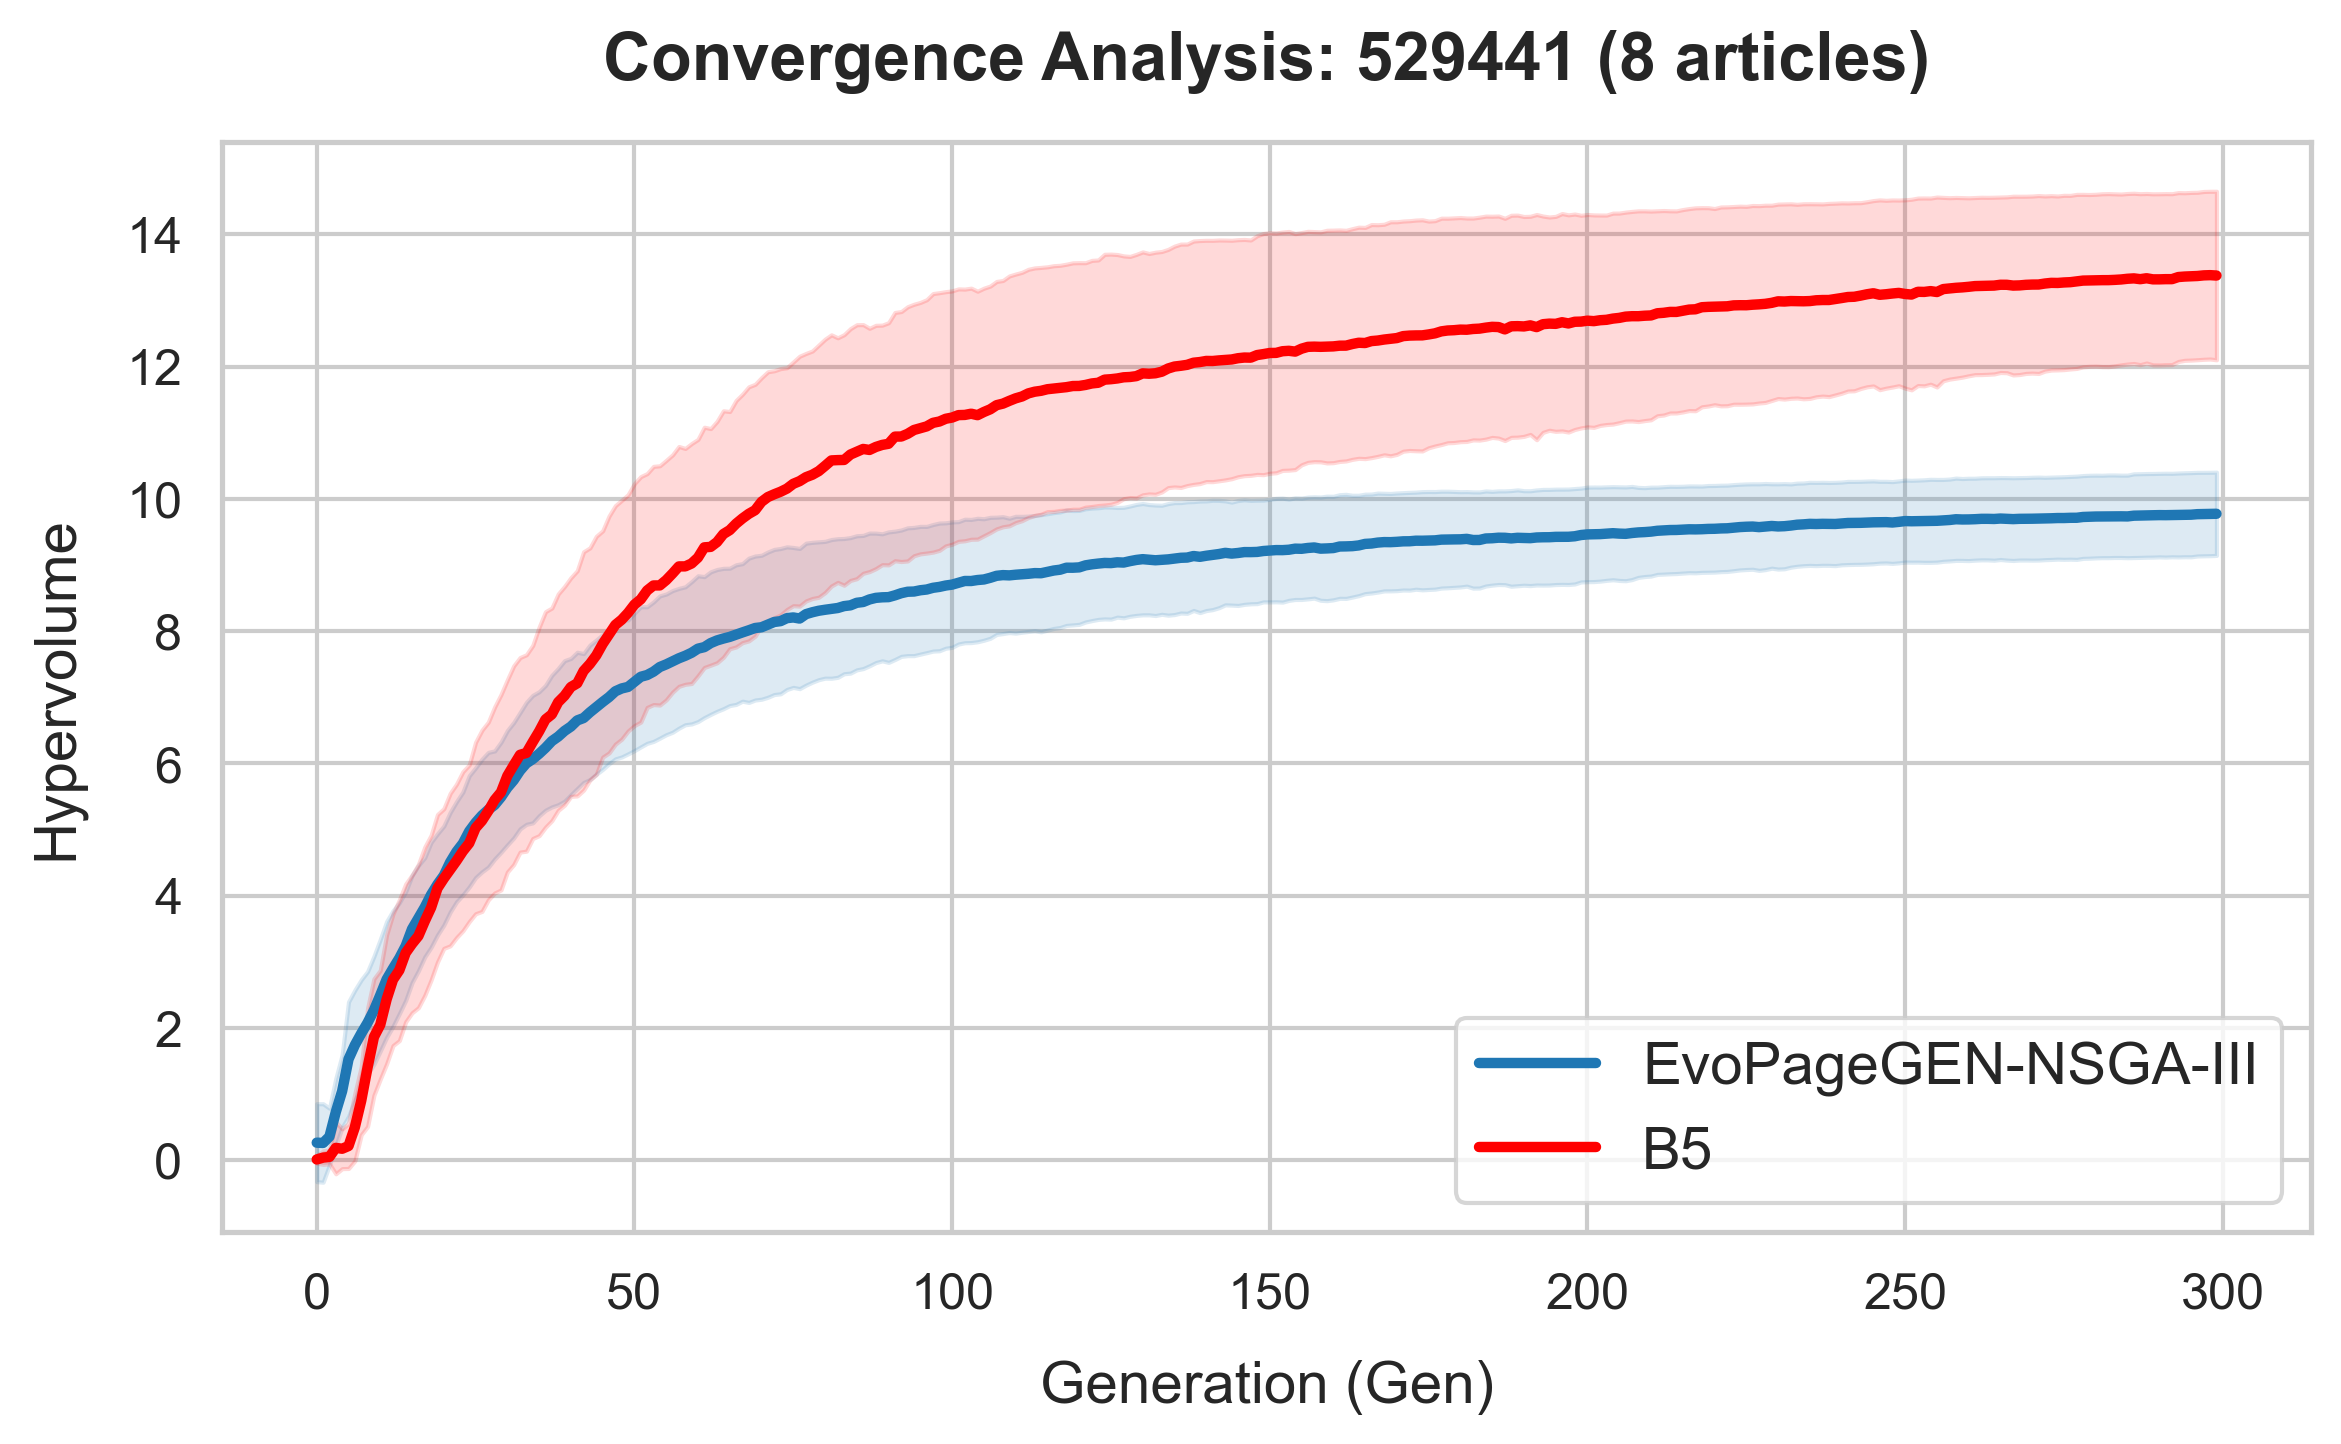
\includegraphics[width=\widthForOneImage]{img/results/convergence_curve.png} 
\caption{Generational convergence analysis tracking the full hypervolume over 300 generations for a highly constrained instance ($\numarticles=8$). Solid lines represent the mean trajectory across all independent runs, while the shaded regions denote the standard deviation.}
\label{fig:convergence_analysis}
\end{figure}

As illustrated in \figref{fig:convergence_analysis}, both methods reach a stable optimization plateau well before the $\ngen$ threshold.

Interestingly, for this specific high-density instance, the ablated baseline ($\baseline{5}$) converges toward a higher average hypervolume. However, it is critical to note that this behavior does not reflect the general performance, as will be demonstrated in the following subsection.

\paragraph{Frontier Size}

Table~\ref{tab:frontier-size} reports the resulting Pareto frontier size for both methods, measured as the number of unique non-dominated solutions, across the evaluated article-count strata.

\begin{table}[htbp]
\centering
\begin{tabular}{lll}
\toprule
\numarticles & $\baseline{5}$ & \methodNameUniform \\
\midrule
2 & 2.0 $\pm$ 1.1 & \bfseries25.0 $\pm$ 8.7 \\
3 & 6.0 $\pm$ 2.6 & \bfseries61.6 $\pm$ 22.2 \\
4 & 10.3 $\pm$ 5.4 & \bfseries98.9 $\pm$ 17.3 \\
5 & 17.2 $\pm$ 7.9 & \bfseries95.7 $\pm$ 28.5 \\
6 & 18.9 $\pm$ 6.3 & \bfseries123.0 $\pm$ 12.9 \\
8 & 25.9 $\pm$ 10.4 & \bfseries77.0 $\pm$ 18.6 \\
\bottomrule
\end{tabular}


\caption{Pareto non-dominated frontier size, defined by the number of unique non-dominated solutions. Metrics express the $\text{mean} \pm \text{standard deviation}$ stratified by article count ($\numarticles$).}
\label{tab:frontier-size}
\end{table}


As shown in Table~\ref{tab:frontier-size}, transitioning from the ablated baseline ($\baseline{5}$) to \methodNameUniform\ expands non-dominated frontier cardinality across all strata, peaking at $123.0 \pm 12.9$ solutions for $n = 6$. This growth was expected, since adding one more objective, \neuralmethod\ ($\objtwo$), to the three already optimized by $\baseline{5}$ ($\objone$, $\objthree$, $\objfour$) mechanically admits more valid trade-off solutions.
However, the magnitude of the increase, up to an order of magnitude larger than $\baseline{5}$'s frontier size in several strata, is far from marginal: it indicates that \objtwo\ introduces substantial tension with the other three objectives, since optimizing human editorial style directly conflicts with tight layout configurations, generating a vast space of valid localized trade-offs.
In practical terms, however, this creates a problem for the intended application: an oversized frontier imposes a considerable cognitive overhead on users who must ultimately select a single layout. This practical bottleneck directly motivates the introduction of a reference-point-guided variant (\methodName), detailed in \secref{sec:rnsga-vs-nsga}.


\paragraph{Hypervolume}

Table~\ref{tab:hv-comparison} reports the resulting Hypervolume (HV) values for both multi-objective methods, evaluated over the full 4D objective space and, separately, over the reduced 3D subspace that excludes \objtwo, across the evaluated article-count strata. Since $\baseline{5}$ never optimizes for $\objtwo$, its value of $\objtwo$ in the 4D space is computed post hoc on its final solutions, without being part of its optimization process.

\begin{table}[htbp]
\centering

\begin{tabular}{lcccc}
\toprule
 & \multicolumn{2}{c}{Full 4D Objective Space ($\objvector$)} & \multicolumn{2}{c}{3D Objective Space (Excluding $\objtwo$)} \\
$\numarticles$ & $\baseline{5}$ & \methodNameUniform & $\baseline{5}$ & \methodNameUniform \\
\midrule
2 & 0.58 $\pm$ 0.36 & \bfseries 1.32 $\pm$ 0.77 & \bfseries 0.72 $\pm$ 0.41 & \bfseries 0.72 $\pm$ 0.41 \\
3 & 2.95 $\pm$ 1.57 & \bfseries 5.63 $\pm$ 2.72 & 1.93 $\pm$ 0.92 & \bfseries 1.96 $\pm$ 0.94 \\
4 & 4.02 $\pm$ 1.40 & \bfseries 8.43 $\pm$ 1.77 & 2.40 $\pm$ 0.47 & \bfseries 2.45 $\pm$ 0.52 \\
5 & 5.03 $\pm$ 2.18 & \bfseries 10.99 $\pm$ 2.55 & 2.64 $\pm$ 0.62 & \bfseries 2.73 $\pm$ 0.60 \\
6 & 5.85 $\pm$ 1.97 & \bfseries 17.17 $\pm$ 0.95 & 3.77 $\pm$ 0.24 & \bfseries 3.85 $\pm$ 0.19 \\
\rowcolor{gray!10} 8 & 4.42 $\pm$ 0.91 & \bfseries 9.77 $\pm$ 0.64 & \bfseries 1.53 $\pm$ 0.15 & 1.49 $\pm$ 0.07 \\
\bottomrule
\end{tabular}

\caption{Hypervolume (HV) quality analysis. The left block evaluates the full 4D objective space. The right block projects the solutions onto the ablated 3D space (excluding $\objtwo$) to assess whether optimizing for editorial style compromises performance. Metrics express the $\text{mean} \pm \text{standard deviation}$. The shaded row ($\numarticles=8$) corresponds to the representative instance tracked in \figref{fig:convergence_analysis}.}
\label{tab:hv-comparison}
\end{table}



As shown in Table~\ref{tab:hv-comparison}, in the full 4D space $(\objone, \objtwo, \objthree, \objfour)$, \methodNameUniform\ exhibits absolute dominance over $\baseline{5}$ across all complexity strata, a direct consequence of successfully integrating the neural editorial style score ($\objtwo$). A Wilcoxon signed-rank test statistically confirms this disparity, yielding an absolute rejection of the null hypothesis ($W = 0.00$, $p < 0.001$, effect size $r = 1.10$). This comparison is nonetheless unfair to $\baseline{5}$, since it is ablated and never optimizes for $\objtwo$ at all; consequently, the right-hand columns of Table~\ref{tab:hv-comparison} restrict the comparison to the reduced 3D objective subspace $(\objone, \objthree, \objfour)$ for which $\baseline{5}$ was originally designed.

This confirms that the tension introduced by \objtwo\ is real and that it helps rather than harms the search: instead of degrading $\objone$, $\objthree$, and $\objfour$, \methodNameUniform\ still consistently matches, and in several strata even outperforms, $\baseline{5}$ within this reduced 3D subspace, a result confirmed by a Wilcoxon signed-rank test ($W = 102.00$, $p = 0.0366$, effect size $r = 0.38$). This regularizing effect forces the population to discover trade-offs that $\baseline{5}$, confined to only three objectives, fails to exploit.

%\paragraph{$\mathcal{C}$-metric}



%\begin{table}[]
  %  \centering
  %  \begin{tabular}{lll}
%\toprule
 %\numarticles & $\mathcal{C}(\text{\methodNameUniform}, \baseline{5})$ & $\mathcal{C}(\baseline{5}, \text{\methodNameUniform})$ \\
%\midrule
%2 & 30.9\% $\pm$ 38.1\% & 1.3\% $\pm$ 3.2\% \\
%3 & 37.1\% $\pm$ 32.7\% & 1.6\% $\pm$ 3.6\% \\
%4 & 35.5\% $\pm$ 31.7\% & 2.4\% $\pm$ 4.9\% \\
%5 & 54.3\% $\pm$ 33.2\% & 1.1\% $\pm$ 2.9\% \\
%6 & 35.4\% $\pm$ 27.6\% & 2.3\% $\pm$ 4.1\% \\
%8 & 48.4\% $\pm$ 32.7\% & 0.1\% $\pm$ 0.8\% \\
%\bottomrule
%\end{tabular}
%\caption{Coverage Metric ($\mathcal{C}$-metric) directional analysis. $\mathcal{C}(A, B)$ expresses the mean percentage of layout solutions in frontier $B$ that are strictly dominated by at least one solution in frontier $A$. Metrics express the $\text{mean} \pm \text{standard deviation}$.}
 %   \label{tab:c_metric_comparison}
%\end{table}

%To finalize the frontier quality evaluation, Table~\ref{tab:c_metric_comparison} presents the bidirectional Coverage Metric ($\mathcal{C}$-metric) to quantify the precise extent of directional dominance between both simultaneous methods. The empirical data reveals a massive asymmetry between the two non-dominated sets. The coverage vector $\mathcal{C}(\text{\methodNameUniform}, \baseline{5})$ consistently invalidates a large proportion of $\baseline{5}$'s generated solutions. 

%This behavior completes the diagnostic established by the previous metrics: \methodNameUniform\ does not simply expand the cardinality of the trade-off set by multiplying redundant configurations, nor does it achieve higher HV by merely pushing boundaries in a single dimension. Instead, \methodNameUniform\  establishes a clear structural dominance over $\baseline{5}$ objective space. The solutions found by embedding the Transformer-guided style score ($\objtwo$) consistently reach coordinates that are unconditionally superior, proving that layouts optimized alongside the space of objectives hold a absolute evolutionary advantage.


\subsubsection{Execution Time Evaluation}
The computational execution time across the evaluated instances, as shown in Table~\ref{tab:exec_time_analysis}, reveals three trends:

\begin{itemize}
    \item $\baseline{1}$ and $\baseline{2}$ are naturally instantaneous since they completely bypass global combinatorial search.
    \item $\baseline{3}$ and $\baseline{4}$ are fast for small pages, but their runtime increases considerably in the largest instance ($\numarticles=8$) due to the $\numarticles!$ permutation bottleneck. At this scale, they approach the execution times of population-based methods, making exact backtracking less attractive for high-density layouts.
    \item Evolutionary methods ($\baseline{5}$ and \methodNameUniform) demand more computational effort. The proposed \methodNameUniform exhibits the highest execution time due to the online neural inference required by \neuralmethod.
\end{itemize}

\begin{table}[htbp]
\centering

\begin{tabular}{lll}
\toprule
$\numarticles$ & Method & Time \\
\midrule
\multirow[c]{6}{*}{2} & B1 & \bfseries 0.003s $\pm$ 0.001s \\
 & B2 & 0.004s $\pm$ 0.001s \\
 & B3 & 0.004s $\pm$ 0.000s \\
 & B4 & 0.006s $\pm$ 0.001s \\
 & B5 & 24.720s $\pm$ 1.330s \\
 & \methodNameUniform & 56.191s $\pm$ 1.052s \\
 \hline
\multirow[c]{6}{*}{3} & B1 & \bfseries0.004s $\pm$ 0.000s \\
 & B2 & \bfseries0.004s $\pm$ 0.000s \\
 & B3 & 0.007s $\pm$ 0.001s \\
 & B4 & 0.009s $\pm$ 0.001s \\
 & B5 & 28.467s $\pm$ 1.072s \\
 & \methodNameUniform & 59.333s $\pm$ 1.659s \\
  \hline
\multirow[c]{6}{*}{4} & B1 & \bfseries0.004s $\pm$ 0.001s \\
 & B2 & 0.005s $\pm$ 0.000s \\
 & B3 & 0.019s $\pm$ 0.002s \\
 & B4 & 0.022s $\pm$ 0.003s \\
 & B5 & 32.902s $\pm$ 1.473s \\
 & \methodNameUniform & 64.299s $\pm$ 1.435s \\
  \hline
\multirow[c]{6}{*}{5} & B1 &\bfseries 0.005s $\pm$ 0.000s \\
 & B2 & \bfseries0.005s $\pm$ 0.000s \\
 & B3 & 0.098s $\pm$ 0.013s \\
 & B4 & 0.100s $\pm$ 0.012s \\
 & B5 & 35.909s $\pm$ 0.796s \\
 & \methodNameUniform & 76.739s $\pm$ 1.799s \\
  \hline
\multirow[c]{6}{*}{6} & B1 & 0.006s $\pm$ 0.003s \\
 & B2 & \bfseries0.005s $\pm$ 0.000s \\
 & B3 & 0.709s $\pm$ 0.020s \\
 & B4 & 0.722s $\pm$ 0.025s \\
 & B5 & 39.517s $\pm$ 0.694s \\
 & \methodNameUniform & 80.614s $\pm$ 0.832s \\
  \hline
\multirow[c]{6}{*}{8} & B1 & \bfseries0.006s $\pm$ 0.000s \\
 & B2 & 0.007s $\pm$ 0.000s \\
 & B3 & 52.710s $\pm$ 0.652s \\
 & B4 & 31.929s $\pm$ 0.521s \\
 & B5 & 48.272s $\pm$ 0.550s \\
 & \methodNameUniform & 90.456s $\pm$ 1.839s \\
\bottomrule
\end{tabular}

\caption{Computational runtime performance across different \numarticles\ strata.}
\label{tab:exec_time_analysis}
\end{table}

Despite this overhead, the execution time remains well within standard industry tolerances, as newspaper layout production does not require real-time processing. As demonstrated in the preceding analysis, this time investment is highly justified by the superior quality and diverse set of alternative Pareto solutions generated, moving away from rigid single-solution outputs. Additionally, potential runtime optimization strategies are deferred to the discussion section.

\subsection{\methodName\ versus \methodNameUniform}
\label{sec:rnsga-vs-nsga}


While \methodNameUniform\ effectively maps the multi-objective space, its uniform selection triggers a combinatorial explosion of the non-dominated frontier. In a production environment, this vast volume of non-dominated solutions imposes a considerable cognitive overhead on human users. To resolve this operational bottleneck, \methodName\ introduces a preference-guided evolutionary paradigm. 

To evaluate both approaches pragmatically, a multi-dimensional Acceptability Envelope (AE) was defined, which serves as an ``envelope'' for solutions that achieves acceptable scores in all objectives, conditioned on the article count $\numarticles$. Rather than relying on arbitrary thresholds, the boundaries of the AE are empirically derived by calculating the 90th percentile ($0.9$ quantile) of the empirical historical distributions for each individual objective ($\objone, \objtwo, \objthree, \objfour$). This section evaluates the total number of generated solutions alongside the exact percentage that successfully falls within the defined AE.


\subsubsection{Pareto Frontier Cardinality}

\begin{table}[htbp]
    \centering
    \begin{tabular}{lll}
\toprule
$\numarticles$ & \methodNameUniform & \methodName \\
\midrule
2 & 25.0 $\pm$ 8.7 & \bfseries5.5 $\pm$ 2.2 \\
3 & 61.6 $\pm$ 22.2 & \bfseries 8.1 $\pm$ 2.9 \\
4 & 98.9 $\pm$ 17.3 & \bfseries13.7 $\pm$ 6.0 \\
5 & 95.7 $\pm$ 28.5 &\bfseries 11.5 $\pm$ 6.5 \\
6 & 123.0 $\pm$ 12.9 & \bfseries17.9 $\pm$ 11.4 \\
8 & 77.0 $\pm$ 18.6 & \bfseries6.2 $\pm$ 2.8 \\
\bottomrule
\end{tabular}
\caption{Comparison of Pareto frontier cardinality. Metrics express the $\text{mean} \pm \text{standard deviation}$, stratified by article count ($\numarticles$).}    \label{tab:frontier_cardinality_comparison}
\end{table}

As outlined in Table~\ref{tab:frontier_cardinality_comparison}, transitioning from the uniform approach to \methodName\ triggers a drastic compression of the non-dominated frontier cardinality across all complexity strata. While \methodNameUniform\ peaks at an average of $123.0 \pm 12.9$ layouts for $\numarticles=6$, the preference-guided mechanism restricts the frontier to a lean, manageable portfolio ranging from $5.5 \pm 2.2$ to $17.9 \pm 11.4$ solutions. 

This contraction is the direct consequence of \methodName's reference-point pruning. By explicitly weighting the evolutionary survival selection toward the historical aspirations, \methodName\ systematically discards operationally unviable areas of the search space. Consequently, this targeted reduction eliminates the severe cognitive overhead imposed on human editors, transforming the multi-objective algorithm from an overwhelming theoretical generator into a highly specialized decision-making tool.


\subsubsection{Percentage of Pareto Frontier within the AE}

\begin{table}[]
    \centering
    \begin{tabular}{lll}
\toprule
$\numarticles$ & \methodNameUniform & \methodName \\
\midrule
2 & 53.8\% $\pm$ 18.5\% & \bfseries74.4\% $\pm$ 20.4\% \\
3 & 68.9\% $\pm$ 18.2\% & \bfseries86.0\% $\pm$ 12.1\% \\
4 & 24.7\% $\pm$ 11.2\% & \bfseries73.5\% $\pm$ 14.2\% \\
5 & 7.5\% $\pm$ 10.5\% & \bfseries34.7\% $\pm$ 26.4\% \\
6 & 6.7\% $\pm$ 3.3\% & \bfseries58.1\% $\pm$ 17.8\% \\
8 & 9.2\% $\pm$ 7.2\% & \bfseries47.1\% $\pm$ 24.3\% \\
\bottomrule
\end{tabular}
\caption{Percentage pareto frontier within the Acceptability Envelope (AE). Metrics express the $\text{mean} \pm \text{standard deviation}$ of the percentage of final non-dominated solutions.}    \label{tab:roi_density_comparison}
\end{table}

The density of solutions within the AE in Table~\ref{tab:roi_density_comparison} confirms the mechanism behind the frontier compression. As instance complexity scales ($\numarticles \ge 4$), the uniform paradigm suffers a severe convergence collapse, with its AE density dropping to single-digit efficiency. This drop mathematically proves that standard uniform environmental selection wastes massive computational budget exploring unviable regions.


Conversely, \methodName\ successfully counteracts this. By anchoring the survival selection around preference-derived aspiration points, \methodName\ concentrates its population within the target zone, maintaining remarkably high densities ($58.1\%$ at $\numarticles=6$ and $47.1\%$ at $\numarticles=8$). When cross-referenced with the cardinality reduction shown in Table~\ref{tab:frontier_cardinality_comparison}, these results deliver a definitive conclusion: \methodName\ does not suffer from a loss of valuable diversity, but rather performs a highly targeted pruning of non-viable space, ensuring the generated alternatives are strictly tailored to the newsroom's operational requirements. To confirm this behavioral shift, a Wilcoxon signed-rank test across all instances was conducted. The test decisively rejects the null hypothesis ($W = 5.0$, $p < 0.001$, effect size of $r = 1.03$), validating that the AE density superiority of \methodName\ is statistically significant.


\begin{figure}[htbp]
\centering
    \begin{subfigure}{\columnwidth}
      \centering
      %todo: put boxplots here to highlight both aspirations points and AE. Refer to section where asp points are defined. put boxplots directly in the graph
      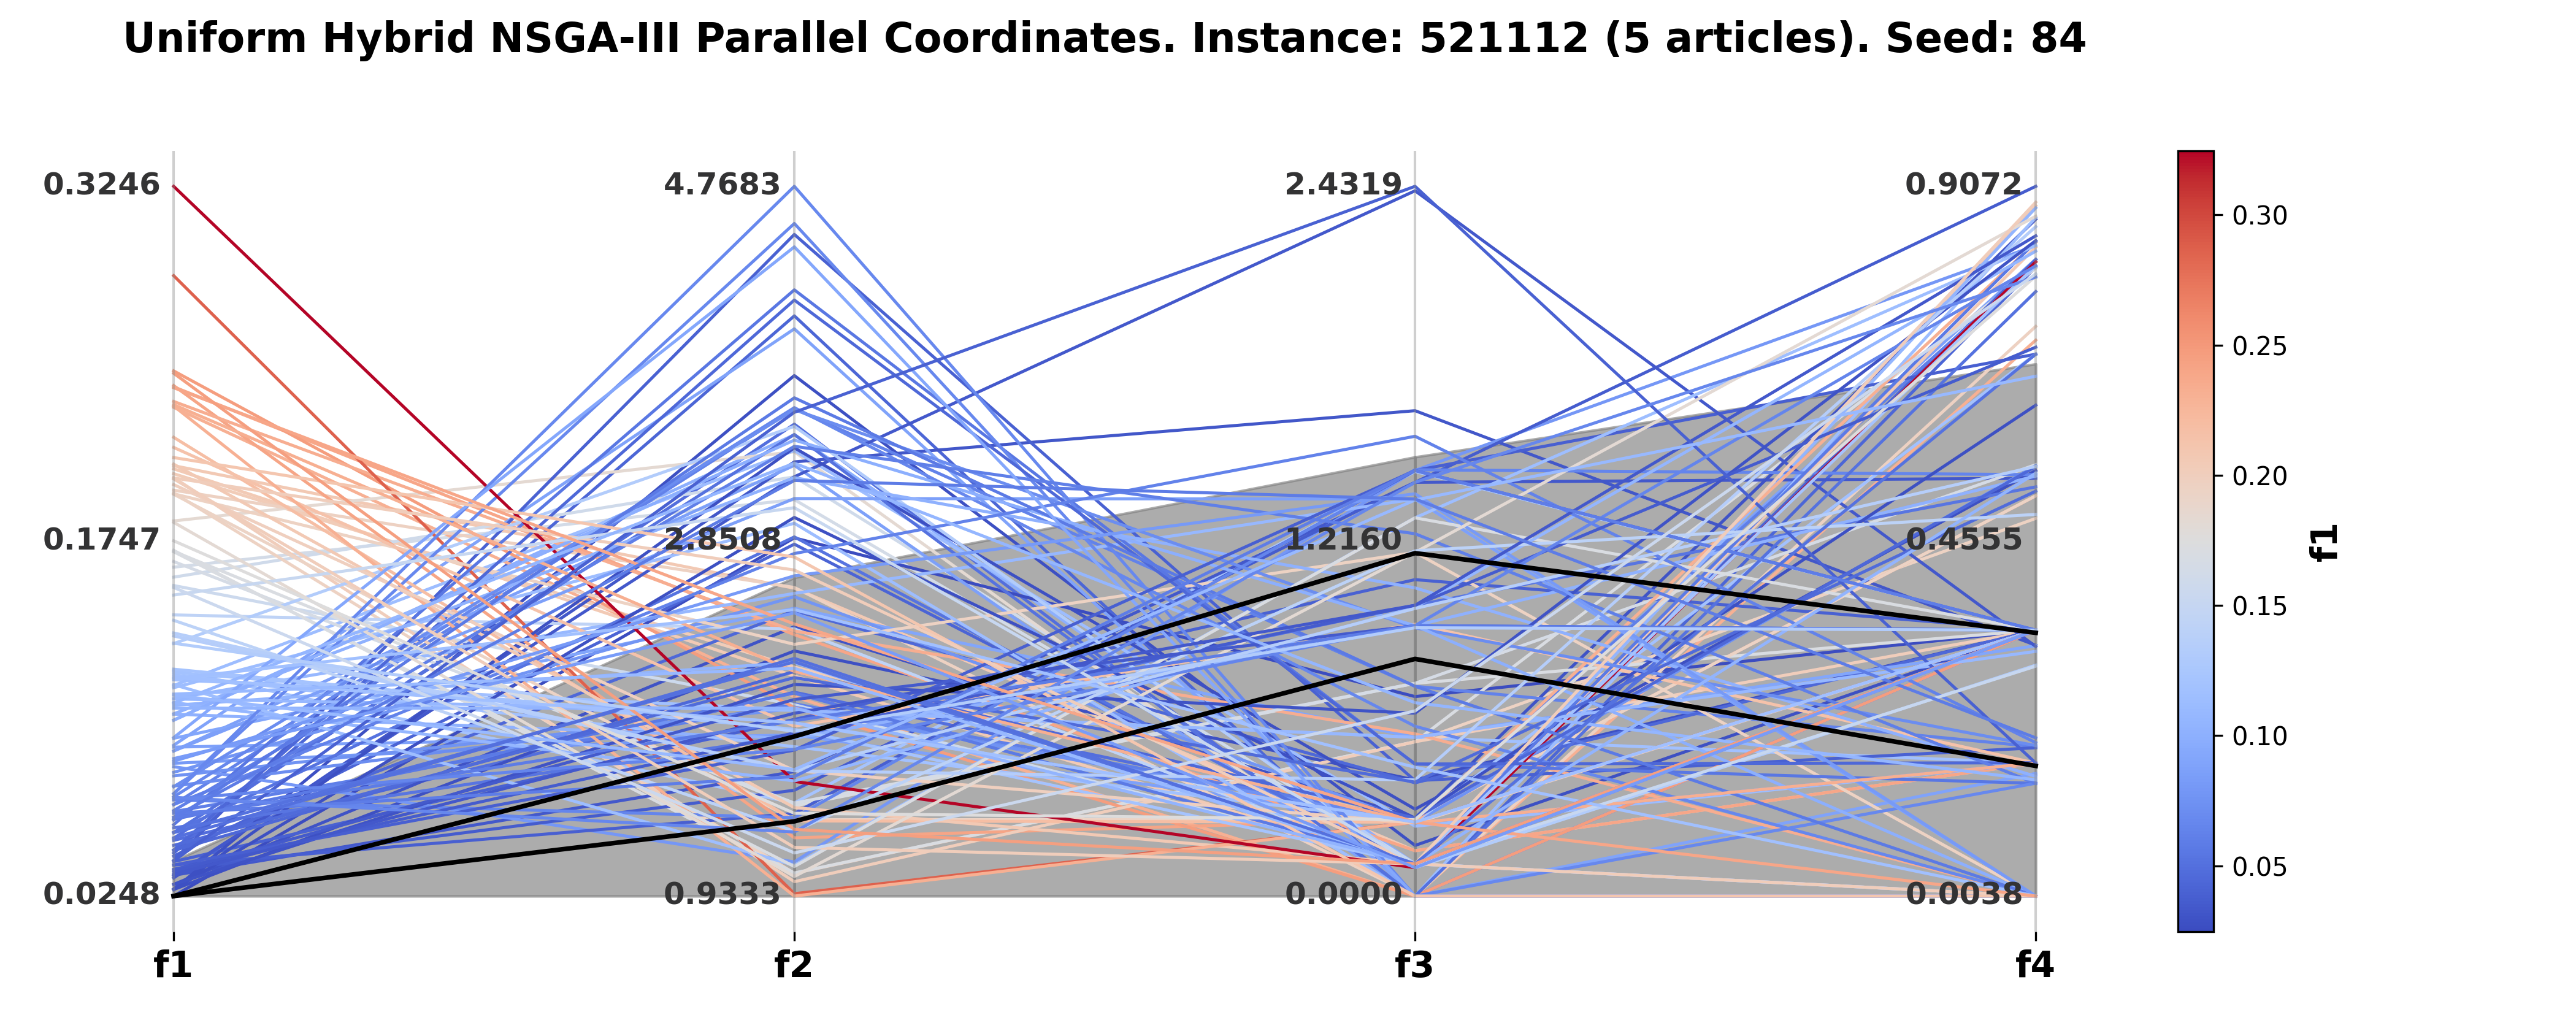
\includegraphics[width=\widthForOneImage]{img/results/nsga_parallel_coordinates_521112_seed_84.png} 
      \caption{\methodNameUniform}
      \label{fig:parallel_uniform}
    \end{subfigure}
    \vspace{0.3cm} % Espaciado controlado entre ambos paneles
    \begin{subfigure}{\columnwidth}
      \centering
      %todo: put boxplots here to highlight both aspirations points and AE. Refer to section where asp points are defined. put boxplots directly in the graph
      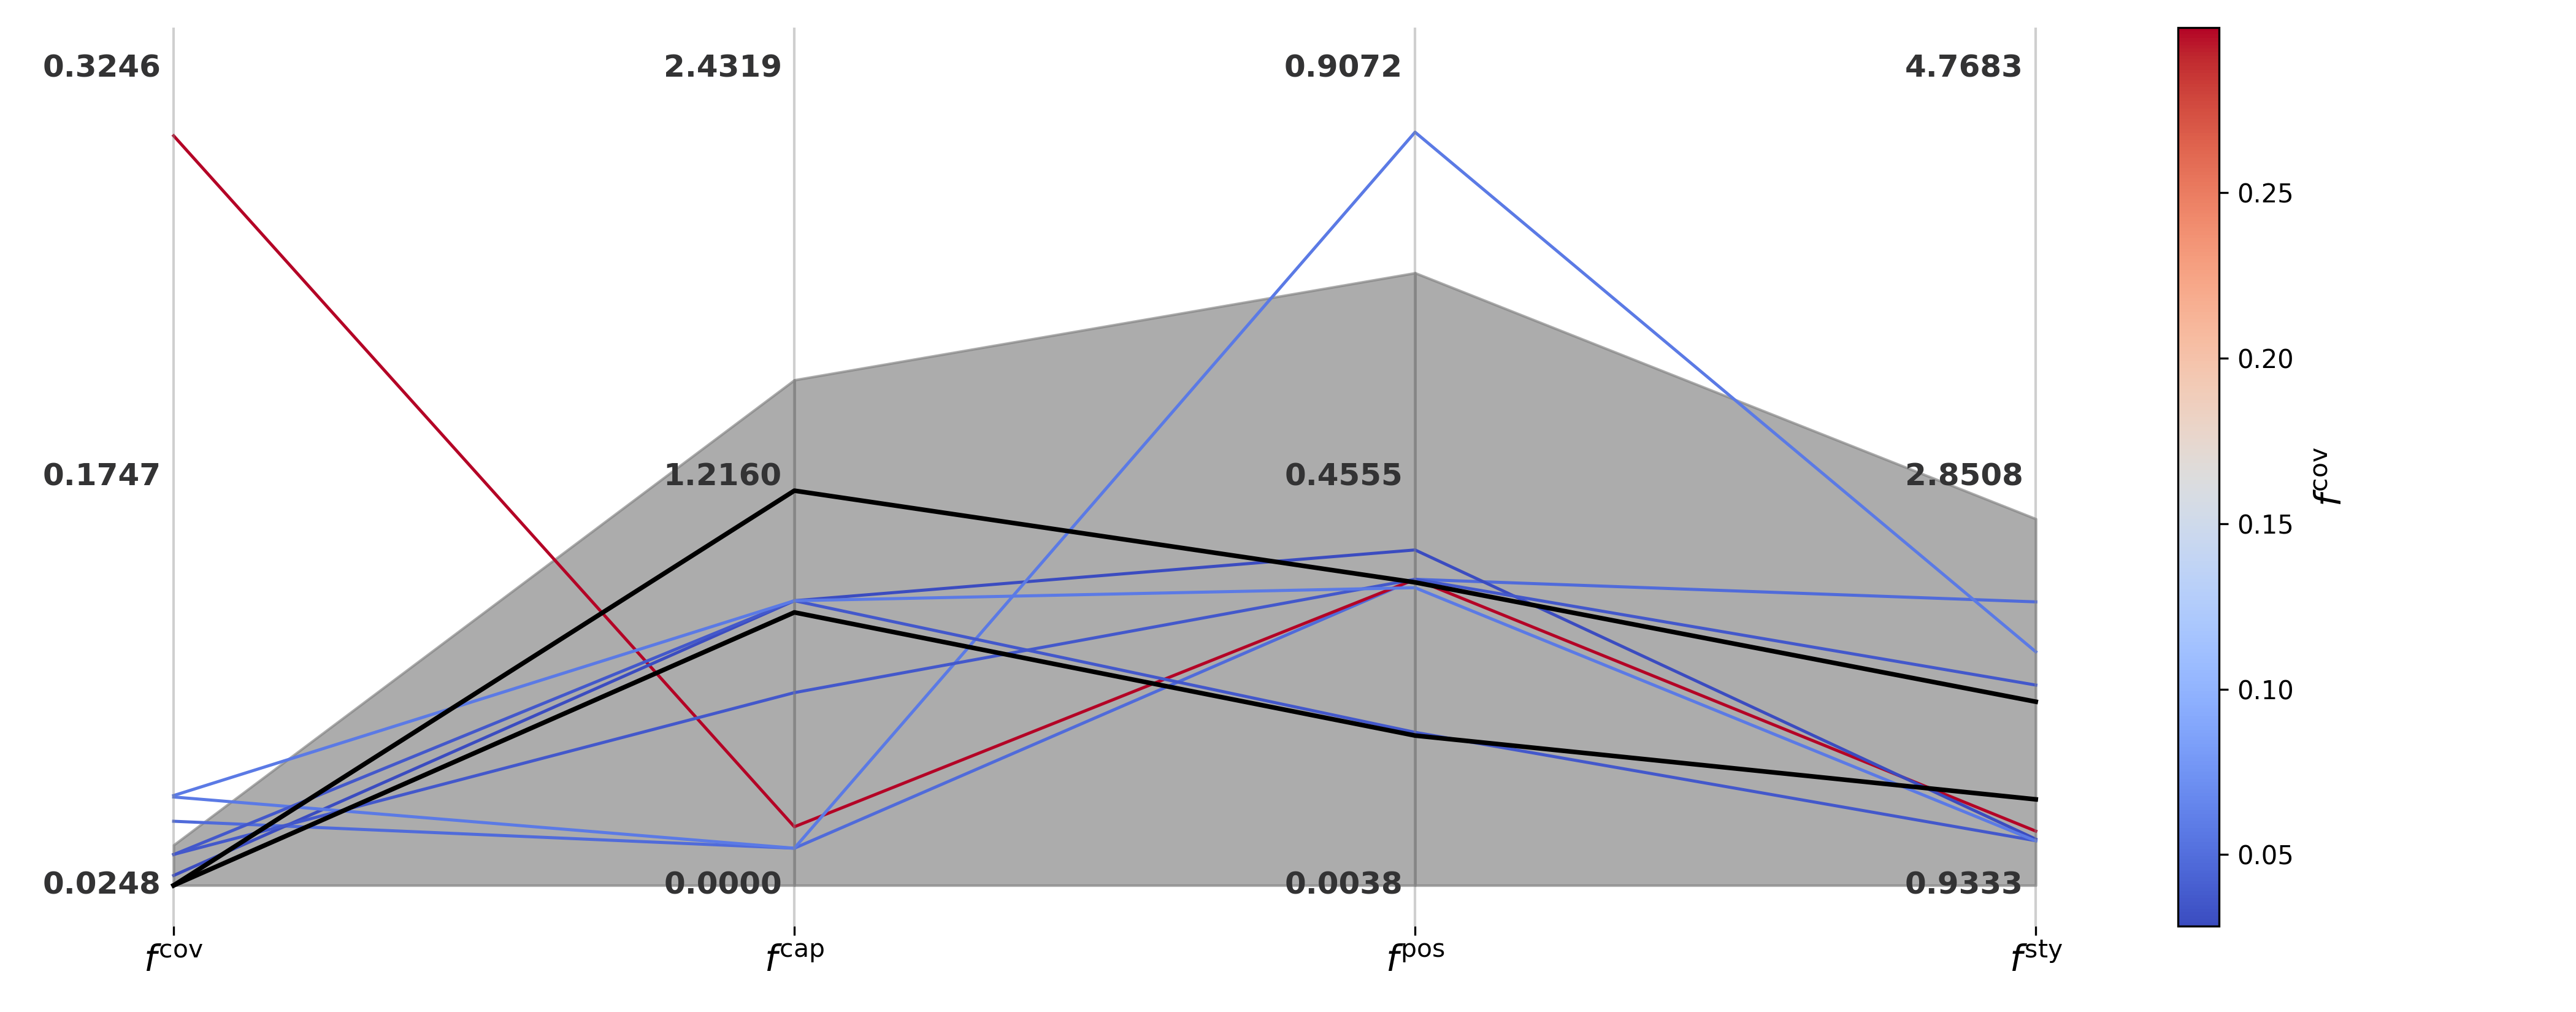
\includegraphics[width=\widthForOneImage]{img/results/rnsga_parallel_coordinates_521112_seed_84.png} 
      \caption{\methodName}
      \label{fig:parallel_rnsga}
    \end{subfigure}
\caption{Visual trade-off comparison using parallel coordinates for a representative medium-complexity instance ($\numarticles=5$) under shared global axis scaling. The gray shaded region represents the AE, while the black lines denote the aspiration points targeted by \methodName. The color gradient reflects the performance on $\objone$. (a) shows \methodNameUniform's non-dominated solutions scattered widely across the objective space, largely outside the AE; (b) shows \methodName's solutions concentrated within the AE, closely following the targeted aspiration points.}
\label{fig:parallel_coordinates_comparison}
\end{figure}


To visually compare frontier size and AE density, \figref{fig:parallel_coordinates_comparison} contrasts the final non-dominated populations of both paradigms for a representative instance ($\numarticles=5$). As shown in \figref{fig:parallel_uniform}, \methodNameUniform's solutions are scattered across the objective space, with many trajectories falling outside the AE, particularly along editorial style ($\objtwo$). This is considered a waste of resources by \methodNameUniform.

In contrast, \figref{fig:parallel_rnsga} shows that \methodName's solutions collapse into a small set of design paths confined to the viable regions of each axis. By discarding operationally unviable layouts, \methodName\ narrows the theoretical Pareto frontier down to a practical set of decision-ready alternatives. This pruning behavior generalizes beyond the specific aspiration points used here, since \methodName\ would concentrate the frontier around any alternative aspiration points. However, generating them using historically grounded targets, as done in this method, is what ensures the resulting alternatives remain aligned with real editorial practice.


\subsubsection{Execution Time}

Beyond frontier cardinality and AE density, both paradigms also differ in computational cost. Table~\ref{tab:exec_time_rnsga_comparison} contrasts their execution times across the same article count strata, where the values reported for \methodNameUniform\ correspond to those already presented in Table~\ref{tab:exec_time_analysis}.


\begin{table}[htbp]
    \centering
    \begin{tabular}{lll}
\toprule
$\numarticles$ & \methodNameUniform & \methodName \\
\midrule
2 & 56.191s $\pm$ 1.052s & 68.52s $\pm$ 1.44s\\
3 & 59.333s $\pm$ 1.659s & 71.86s $\pm$ 2.11s\\
4 & 64.299s $\pm$ 1.435s & 78.47s	$\pm$ 1.79s\\
5 & 76.739s $\pm$ 1.799s & 93.83s	$\pm$ 2.97s\\
6 & 80.614s $\pm$ 0.832s & 99.21s	$\pm$ 2.27s\\
8 & 90.456s $\pm$ 1.839s & 111.77s $\pm$ 2.01s\\
\bottomrule
\end{tabular}
\caption{Execution time comparison between the uniform and the preference-guided paradigms. The values reported for \methodNameUniform\ are reproduced from Table~\ref{tab:exec_time_analysis}. Metrics express the $\text{mean} \pm \text{standard deviation}$, stratified by article count ($\numarticles$).}
\label{tab:exec_time_rnsga_comparison}
\end{table}

The measurements reveal that \methodName\ incurs a systematically higher execution time than \methodNameUniform, with an overhead comprised between $21\%$ and $24\%$ across the evaluated strata. This penalty can be explained by two reasons: 

\begin{enumerate}
  \item The population size is higher. \methodName\ evolves $\popsize_{R} = 330$ individuals against $\popsize = 286$, which amounts to $15.4\%$ additional chromosome decodings per generation. 
  \item The survival selection mechanism itself. The reference-point niching of \methodName\ must evaluate the distance of every individual to each of the local reference directions generated around the aspiration points and contracted by $\RNSGAradius$, an operation more costly than the single, global association against the uniform Das-Dennis mesh employed by \methodNameUniform.
\end{enumerate}

Two properties of this overhead deserve to be noted. First, it remains proportionally stable across the complexity strata instead of degrading as the article count grows, which indicates that the additional cost scales with the population and the selection mechanism rather than with the combinatorial difficulty of the instance. Second, the most demanding instance evaluated ($\numarticles = 8$) is still resolved in $111.77$s, hence below two minutes per page. The preference-guided paradigm of \methodName\ therefore justify its operational advantages, namely a frontier reduced by an order of magnitude and a substantially higher density within the acceptability envelope, at a bounded and predictable computational time, which is acceptable in a production setting where page building is not a real-time task. These runtimes correspond to the reference configuration reported in \secref{sec:implementation_details}; on less capable hardware the absolute values scale accordingly, in which case the mitigation strategies examined in \secref{sec:computational-performance} become directly applicable.


\subsection{Comparison with input}
%todo do a pareto dominance analysis and maybe knee point

\subsection{Qualitative results}

To complement the quantitative evaluation, this section provides a few examples of the pages synthesized by the framework. \figref{fig:qualitative_2art}, \figref{fig:qualitative_4art}, \figref{fig:qualitative_5art}, and \figref{fig:qualitative_8art} present four representative instances of increasing complexity ($\numarticles = 2, 4, 5, 8$). For each instance, the original input page is shown alongside three design alternatives (A, B, C) drawn from the non-dominated frontier produced by \methodName, together with their corresponding objective scores ($\objone, \objthree, \objfour, \objtwo$), visually illustrating the structural diversity and design plasticity achieved by \methodName.

It must be emphasized that the original input page displayed in each figure is included solely as a visual reference, corresponding to the real, human-designed page available for that instance within \laprovence archive. This layout is never observed by \methodName\. The optimization method only receives the formal input vector $\instance = \langle \page, \articleset \rangle$, that is, the article content and page constraints, while every geometric coordinate, template assignment, and positioning decision is stripped prior to optimization. Consequently, the objective scores reported for the original input page must not be interpreted as a baseline that \methodName\ is expected to systematically outperform, but merely as a reference illustrating how the same content was historically composed by a human designer, since in a real deployment scenario the original layout would remain entirely unknown to the system.

\begin{figure}[htbp]
\centering
\begin{subfigure}{0.48\widthForOneImage}
  \centering
  
\includegraphics[width=0.85\linewidth]{img/results/examples/compressed/2_art/input_P4_162514.png}\\[2pt]
  {\footnotesize $\objone = 0.00,\ \objthree = 0.37,\ \objfour = 0.00,\ \objtwo = 1.55$}
  \caption{Original Input}
  \label{fig:qual_n2_input}
\end{subfigure}
\hfill
\begin{subfigure}{0.48\widthForOneImage}
  \centering
  
\includegraphics[width=0.85\linewidth]{img/results/examples/compressed/2_art/solution_P4_idx0_162514_page1.png}\\[2pt]
  {\footnotesize $\objone = 0.01,\ \objthree = 0.31,\ \objfour = 0.00,\ \objtwo = 0.55$}
  \caption{Design Alternative A}
  \label{fig:qual_n2_A}
\end{subfigure}

\vspace{0.3cm}

\begin{subfigure}{0.48\widthForOneImage}
  \centering
  
\includegraphics[width=0.85\linewidth]{img/results/examples/compressed/2_art/solution_P4_idx3_162616_page1.png}\\[2pt]
  {\footnotesize $\objone = 0.02,\ \objthree = 0.26,\ \objfour = 0.00,\ \objtwo = 1.11$}
  \caption{Design Alternative B}
  \label{fig:qual_n2_B}
\end{subfigure}
\hfill
\begin{subfigure}{0.48\widthForOneImage}
  \centering
  
\includegraphics[width=0.85\linewidth]{img/results/examples/compressed/2_art/solution_P4_idx6_162621_page1.png}\\[2pt]
  {\footnotesize $\objone = 0.01,\ \objthree = 0.31,\ \objfour = 0.00,\ \objtwo = 0.35$}
  \caption{Design Alternative C}
  \label{fig:qual_n2_C}
\end{subfigure}

\caption{Original input page and three non-dominated design alternatives generated by \methodName\ for a representative instance of complexity $\numarticles=2$, together with their objective scores $\objone, \objthree, \objfour, \objtwo$.}
\label{fig:qualitative_2art}
\end{figure}

\begin{figure}[htbp]
\centering
\begin{subfigure}{0.48\widthForOneImage}
  \centering
  
\includegraphics[width=0.85\linewidth]{img/results/examples/compressed/4_art/input_P4_161909.png}\\[2pt]
  {\footnotesize $\objone = 0.02,\ \objthree = 1.19,\ \objfour = 0.17,\ \objtwo = 1.17$}
  \caption{Original Input}
  \label{fig:qual_n4_input}
\end{subfigure}
\hfill
\begin{subfigure}{0.48\widthForOneImage}
  \centering
  
\includegraphics[width=0.85\linewidth]{img/results/examples/compressed/4_art/solution_P4_idx1_162103_page1.png}\\[2pt]
  {\footnotesize $\objone = 0.04,\ \objthree = 1.56,\ \objfour = 0.34,\ \objtwo = 0.76$}
  \caption{Design Alternative A}
  \label{fig:qual_n4_A}
\end{subfigure}

\vspace{0.3cm}

\begin{subfigure}{0.48\widthForOneImage}
  \centering
  
\includegraphics[width=0.85\linewidth]{img/results/examples/compressed/4_art/solution_P4_idx2_162130_page1.png}\\[2pt]
  {\footnotesize $\objone = 0.05,\ \objthree = 0.26,\ \objfour = 0.34,\ \objtwo = 3.14$}
  \caption{Design Alternative B}
  \label{fig:qual_n4_B}
\end{subfigure}
\hfill
\begin{subfigure}{0.48\widthForOneImage}
  \centering
  
\includegraphics[width=0.85\linewidth]{img/results/examples/compressed/4_art/solution_P4_idx10_161909_page1.png}\\[2pt]
  {\footnotesize $\objone = 0.02,\ \objthree = 0.97,\ \objfour = 0.34,\ \objtwo = 1.63$}
  \caption{Design Alternative C}
  \label{fig:qual_n4_C}
\end{subfigure}

\caption{Original input page and three non-dominated design alternatives generated by \methodName\ for a representative instance of complexity $\numarticles=4$, together with their objective scores $\objone, \objthree, \objfour, \objtwo$.}
\label{fig:qualitative_4art}
\end{figure}

\begin{figure}[htbp]
\centering
\begin{subfigure}{0.48\widthForOneImage}
  \centering
  
\includegraphics[width=0.85\linewidth]{img/results/examples/compressed/5_art/input_P4_162942.png}\\[2pt]
  {\footnotesize $\objone = 0.02,\ \objthree = 6.91,\ \objfour = 0.64,\ \objtwo = 1.77$}
  \caption{Original Input}
  \label{fig:qual_n5_input}
\end{subfigure}
\hfill
\begin{subfigure}{0.48\widthForOneImage}
  \centering
  
\includegraphics[width=0.85\linewidth]{img/results/examples/compressed/5_art/solution_P4_idx1_163007_page1.png}\\[2pt]
  {\footnotesize $\objone = 0.04,\ \objthree = 1.54,\ \objfour = 0.51,\ \objtwo = 2.72$}
  \caption{Design Alternative A}
  \label{fig:qual_n5_A}
\end{subfigure}

\vspace{0.3cm}

\begin{subfigure}{0.48\widthForOneImage}
  \centering
  
\includegraphics[width=0.85\linewidth]{img/results/examples/compressed/5_art/solution_P4_idx3_162942_page1.png}\\[2pt]
  {\footnotesize $\objone = 0.05,\ \objthree = 1.58,\ \objfour = 0.51,\ \objtwo = 2.40$}
  \caption{Design Alternative B}
  \label{fig:qual_n5_B}
\end{subfigure}
\hfill
\begin{subfigure}{0.48\widthForOneImage}
  \centering
  
\includegraphics[width=0.85\linewidth]{img/results/examples/compressed/5_art/solution_P4_idx5_163028_page1.png}\\[2pt]
  {\footnotesize $\objone = 0.06,\ \objthree = 0.66,\ \objfour = 0.34,\ \objtwo = 2.31$}
  \caption{Design Alternative C}
  \label{fig:qual_n5_C}
\end{subfigure}

\caption{Original input page and three non-dominated design alternatives generated by \methodName\ for a representative instance of complexity $\numarticles=5$, together with their objective scores $\objone, \objthree, \objfour, \objtwo$.}
\label{fig:qualitative_5art}
\end{figure}

\begin{figure}[htbp]
\centering
\begin{subfigure}{0.48\widthForOneImage}
  \centering
  
\includegraphics[width=0.85\linewidth]{img/results/examples/compressed/8_art/input_P4_164245.png}\\[2pt]
  {\footnotesize $\objone = 0.04,\ \objthree = 1.33,\ \objfour = 0.17,\ \objtwo = 2.47$}
  \caption{Original Input}
  \label{fig:qual_n8_input}
\end{subfigure}
\hfill
\begin{subfigure}{0.48\widthForOneImage}
  \centering
  
\includegraphics[width=0.85\linewidth]{img/results/examples/compressed/8_art/solution_P4_idx0_164245_page1.png}\\[2pt]
  {\footnotesize $\objone = 0.05,\ \objthree = 0.22,\ \objfour = 0.17,\ \objtwo = 2.99$}
  \caption{Design Alternative A}
  \label{fig:qual_n8_A}
\end{subfigure}

\vspace{0.3cm}

\begin{subfigure}{0.48\widthForOneImage}
  \centering
  
\includegraphics[width=0.85\linewidth]{img/results/examples/compressed/8_art/solution_P4_idx2_164309_page1.png}\\[2pt]
  {\footnotesize $\objone = 0.11,\ \objthree = 0.00,\ \objfour = 0.17,\ \objtwo = 2.10$}
  \caption{Design Alternative B}
  \label{fig:qual_n8_B}
\end{subfigure}
\hfill
\begin{subfigure}{0.48\widthForOneImage}
  \centering
  
\includegraphics[width=0.85\linewidth]{img/results/examples/compressed/8_art/solution_P4_idx4_164428_page1.png}\\[2pt]
  {\footnotesize $\objone = 0.06,\ \objthree = 0.10,\ \objfour = 0.31,\ \objtwo = 2.25$}
  \caption{Design Alternative C}
  \label{fig:qual_n8_C}
\end{subfigure}

\caption{Original input page and three non-dominated design alternatives generated by \methodName\ for a representative instance of complexity $\numarticles=8$, together with their objective scores $\objone, \objthree, \objfour, \objtwo$. }
\label{fig:qualitative_8art}
\end{figure}

A qualitative inspection of \figref{fig:qualitative_2art}--\figref{fig:qualitative_8art} reveals several consistent design patterns in the behavior of \methodName:
\begin{enumerate}
    \item Homogeneous Template Replication: All three design alternatives generated for the highest-density instance ($\numarticles=8$, \ref{fig:qual_n8_A}--\ref{fig:qual_n8_C}) group the majority of their secondary articles into a repeated sequence of the same narrow-column template, regardless of the specific trade-off targeted by each alternative. This consistency across independently sampled solutions of the non-dominated frontier indicates that \methodName\ reliably discovers this journalistic convention of building clean, tabular sections whenever a page must accommodate a large number of short secondary articles.

    \item Improvement over the Human Baseline: Although outperforming the original input page is not the primary goal of \methodName, since its layout is never observed by the method (as discussed above), the generated alternatives frequently improve upon it. This is most apparent for text capacity ($\objthree$): 11 of the 12 alternatives shown across the four instances attain a lower (better) $\objthree$ score than the corresponding input, the only exception being Alternative~\ref{fig:qual_n4_A}. The largest gap is observed for the $\numarticles=5$ instance, where $\objthree$ falls from $6.91$ in the original page to values between $0.66$ and $1.58$ among the three alternatives. A comparable, though less systematic, trend appears for $\objtwo$, most clearly for the $\numarticles=2$ instance, where all three alternatives improve over the input's $\objtwo = 1.55$, down to as low as $0.35$. Wasted space ($\objone$), in contrast, is equal to or higher for the generated alternatives than for the original page in 11 of the 12 cases, which is expected: human designers compose the page with full knowledge of its final layout, whereas \methodName\ operates blindly on content alone and trades a small amount of page occupation efficiency for gains along the remaining objectives.

    \item Pareto-Optimal Trade-offs: \figref{fig:qualitative_5art} illustrates the intrinsically Pareto-optimal nature of the non-dominated frontier explored by \methodName. Among the three alternatives generated for the $\numarticles=5$ instance, Design Alternative~\ref{fig:qual_n5_C} attains the lowest positioning penalty ($\objfour = 0.34$, against $0.51$ for both~\ref{fig:qual_n5_A} and~\ref{fig:qual_n5_B}) and the lowest text capacity penalty ($\objthree = 0.66$, against $1.54$ and $1.58$), at the cost of a visibly lower page occupation efficiency: a small rectangular gap remains unfilled in the lower-left region of the page, raising its wasted space score to $\objone = 0.06$, the highest of the three alternatives ($0.04$ and $0.05$, respectively). This exemplifies how \methodName\ willingly sacrifices a marginal amount of page coverage in exchange for a substantial gain along the remaining dimensions, rather than converging onto a single compromise solution.
\end{enumerate}
Crucially, the system learns and deploys these complex, real-world layout rules spontaneously through preference-guided reference points and a surrogate deep-learning model (\neuralmethod) without requiring explicit procedural constraints, confirming its utility as a flexible layout generation method.

\section{Discussion}
\label{sec:pagegen-discussion}

While the quantitative and qualitative findings validate the efficacy of \methodNameGeneral, two primary aspects require a critical analysis regarding its  industrial deployment, and architectural extensibility.

\subsection{Computational performance and scalability}
\label{sec:computational-performance}
Execution time represents the primary computational bottleneck of \methodNameGeneral\ when contrasted against the constructive baselines, whose runtimes remain in the millisecond range. This overhead is nonetheless bounded: even \methodName, which is the more costly of the two paradigms, resolves the most demanding instance evaluated in under two minutes per page (Table~\ref{tab:exec_time_rnsga_comparison}). 
Beyond this, several optimization approaches can be deployed to further mitigate the overhead in production environments. First, as observed during the convergence analysis, the evolutionary search stabilizes early, around generation 200. Consequently, reducing the total generation horizon ($\ngen$) from $300$ to $200$ generations provides an immediate mechanism to accelerate response times without compromising frontier quality; assuming a cost roughly proportional to the number of generations, this measure alone would bring the most demanding instance from $111.77$s down to approximately $75$s. 
Moreover, since convergence speed itself varies with instance complexity (e.g., lower-density instances such as $\numarticles=5$ already converge faster than the high-density $\numarticles=8$ case analyzed above), adapting $\ngen$ per instance based on observed convergence, rather than applying a single fixed budget across all strata, would yield further speedups.

Second, a more aggressive reduction in execution time can be achieved through concurrent computing. Both the global evolutionary engine and the localized packing decoder are highly susceptible to parallelization. While sequential execution was maintained in this study to eliminate race conditions and ensure deterministic architectural simplicity, deploying a multi-threaded asynchronous pipeline would drastically reduce processing times. However, even under the current sequential configuration, the execution times achieved by \methodNameGeneral\ are already operationally viable within the specific industrial newsroom production environment targeted by this investigation. The most demanding instance evaluated, resolved in $111.77$s by the more costly of the two paradigms, remains within the tolerance of a few minutes per page specified by the industrial partner (\secref{sec:industrial-motivation}), and therefore satisfies the temporal criterion of the main objective stated in \secref{sec:multi-objective-page-generation}, in contrast with the fifteen to twenty minutes of manual editing per page that \melody's current workflow still demands (\secref{sec:industrial-motivation}).

\subsection{Architectural extensibility to advertisement placement}
The current implementation of \methodNameGeneral\ omits the placement of advertisement elements. This omission stems strictly from dataset limitations, as historical layout records lack consistent metadata regarding advertisement coordinates and dimensions. However, the underlying mathematical framework is fully generalizable and capable of incorporating these elements.

To integrate advertisements, these assets can be modeled as static, fixed-size bounding boxes within the chromosome representation. Unlike standard articles, advertisement blocks would bypass the template selection layer, as their aspect ratios are predetermined, and feed directly into the spatial packing decoder. Furthermore, to guide their placement, a localized spatial penalty function can be formulated. This function would operate analogously to the main article zone objective ($\HCZ$), penalizing configurations that displace advertisements outside of the newspaper's historically preferred advertising quadrants. Beyond this parameterization, the core mechanisms of \methodNameGeneral\ remain robust and inherently scalable.

